%!TEX root = ../thesis.tex
%*******************************************************************************
%*********************************** Introduction Chapter *****************************
%*******************************************************************************

\chapter{Introduction}
\graphicspath{{Chapter_Intro/Figs/}}

The pursuit of three-dimensional (3D) display has never stopped. Currently, most commercially available so-called `3D display' products such as 3D cinema, 3D TV, handheld 3D devices (e.g. Nintendo 3DS, HTC Evo 3D) and Virtual Reality (VR) and Augmented Reality (AR) head sets are in fact stereoscopic displays where two different two-dimensional (2D) images are displayed to the left and right eye respectively, creating a 3D illusion in the brain. Despite its high image quality, the major issue with stereoscopic displays is that they cannot provide real defocusing effect in depth. Modern 3D cinema are able to provide good comfort because the polarisation glasses are as light as regular glasses, and the variable defocusing issue can be avoided by the combination of good design of point of interest in each scene and the according defocusing effect as captured by the camera, so most audience won't experience much discomfort for around 2 to 3 hours. But the content, viewing angle and depth of focus are fixed at how they are captured. To provide an interactive and real-time rendered immersive experience, the VR/AR headset has frequently been advertised as the `gateway to metaverse' in recent years. However, my personal experience with VR headset is far from comfortable, not only because of its heavy weight, but also because the display is physically at a very near distance, while my brain thinks the objects are at various distances and yet are still all in focus, which is very unnatural, because in real life, when the eye is focused on a near object, the far backgrounds would blur out. And also, the two displays in the VR headset needs to be rendered in real-time based on the location and angle of the user, which is nowhere near practical. Hence, the heavy weight, the lack of defocusing, the delay between the rendering and the change in my position are the three major factors causing my dizziness using VR headsets, either of which is quite impractical to solve, especially the weight issue. Only if VR/AR headsets could be reduced to the weight of eyeglasses would I ever consider the possibility of those head-mounted devices leading us to the `metaverse'.

In comparison, the holography technique can produce the full 3D light field, which does not rely on any head mounted device, has the true depth of focus, and does not need to re-render according to change in viewer positions and viewing angle.

\begin{figure}[H]
    \centering
    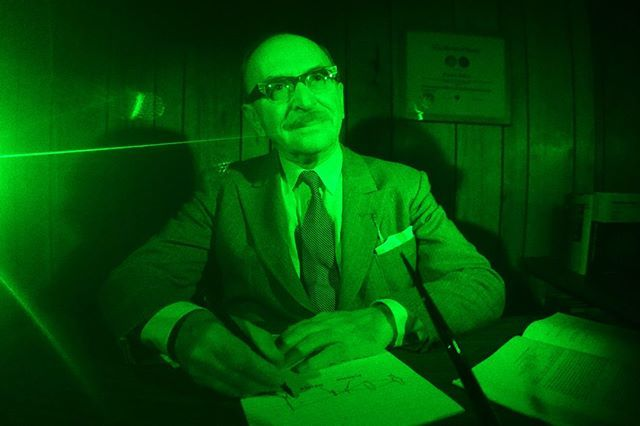
\includegraphics[width=0.6\textwidth]{Dennis-Gabor-Hologram-2.jpg}
    \caption{A photo of the holographic portrait of Dennis Gabor \cite{Lo2018}}\label{fig:Dennis-Gabor-Hologram-2}
\end{figure}

Holography, taking its name from the Greek word $o \lambda o \sigma $ (holos), meaning \textit{whole}, was first introduced in 1948 by Dennis Gabor \cite{Gabor1948}, originally named as \textit{wavefront reconstruction} \cite{Hecht2017}. It is a cool technology which generates 3D images via the diffraction of light. Similar to 2D photography, the earliest holography uses a piece of film to record the diffraction pattern, which can then reconstruct the 3D field, as shown in \cref{fig:Dennis-Gabor-Hologram-2} which is a holographic recording of Dennis Gabor himself. After the invention of digital cameras, digital holography emerged. The limitation of both methods is that they require a physical object as a priori to record the hologram. In order to generate hologram for objects that do not physically exist, computer-generated holography (CGH) emerged where a hologram can be calculated through various algorithmic approaches and then displayed on a spatial light modulator (SLM) modulating the wavefront of a coherent light source in order to produce 3D multi-depth image reconstructions. Currently available SLM's can only modulate either phase or amplitude, so algorithms are needed to compute amplitude-only or phase-only holograms. The classic phase-retrieval algorithms include direct binary search \cite{Seldowitz1987}, simulated annealing \cite{Kirkpatrick1983} and Gerchberg-Saxton \cite{Gerchberg1972}. With the developments in modern numerical optimisation methods and increase in computational power, phase retrieval with new numerical optimisation methods has also been found in the literature such as: gradient descent \cite{Zhang2017, Liu2020}, its stochastic variations \cite{Chen2021, Choi2021, Kadis2022}. However, all the existing phase retrieval methods still has some fundamental issues, mainly their poor image quality and/or the heavy computation required, the solutions of which are my ultimate goals.

This thesis therefore explores the development and optimisation of phase-only CGH for holographic displays. The research investigates various phase retrieval algorithms and proposes novel methods to enhance the reconstruction quality and computational efficiency of hologram, after which it dives into the fundamental limits of the discretised phase holograms on their information capacity. The thesis is structured as following.

Chapter 2 provides a comprehensive literature review, covering the fundamental theories of light, the principles of holography, and the evolution of CGH methods. The chapter reviews various phase retrieval algorithms, including the Naive, Direct Binary Search (DBS), Simulated Annealing (SA), Gerchberg-Saxton (GS), One-Step Phase Retrieval (OSPR), and Adaptive One-Step Phase Retrieval (AD-OSPR) algorithms and their adaptations for 3D CGH, emphasizing the limitations of current algorithms and introducing the motivation for pursuing more advanced CGH techniques.

Chapter 3 proposes the Digital Pre-Distorted One-Step Phase Retrieval (DPD-OSPR) method. By experimentally evaluating the non-linearities in the holographic projection system and applying a digital pre-distortion (DPD) curve, significant improvements in reconstruction quality and reductions in mean squared error are demonstrated.

Chapter 4 introduces the optimisation of phase-only holograms using the Limited-memory Broyden-Fletcher-Goldfarb-Shanno (L-BFGS) optimisation algorithm, and then proposes the novel Target Image Phase Optimisation (TIPO) technique, which optimises the phase of the target image instead of the phase of the hologram. Then the multi-depth phase-only hologram optimisation for 3D targets is investigated, and a novel technique called Sequential Slicing (SS) is proposed, which evaluates the loss for a single slice of the 3D target at each iteration instead of a full evaluation on all slices, reducing computational time while maintaining overall quality and minimizing quality imbalances across all slices.

Chapter 5 extends the optimisation method on generating time-multiplexing binary-phase holograms, and proposes the novel Multi-Frame Holograms Batched Optimisation (MFHBO) technique. By optimising a batch of holograms for time multiplexing, which leverages the finite response time of human vision to average out noise, resulting in improved visual quality. The MFHBO algorithm shows a much better quality than the existing time-multiplexing hologram generation methods such as OSPR and AD-OSPR.

Chapter 6 dives into the information capacity of phase-only CGH. This chapter examines the effects of quantisation on hologram bit depth and their impact on reconstruction quality, and looks for the correlation between the entropy of the target image and the reconstruction error, providing insights into the fundamental limits of discretised CGH.

Chapter 7 marks the conclusion and lists potential further work that could be done.
